%%%%%%%%%%%%%%%%%%%%%%%%%%%%%%%%%%%%%%%%%%%%%%%%%%%%%%%%%%%%%%%%%%%%%%%%%%%%%%%%
%2345678901234567890123456789012345678901234567890123456789012345678901234567890
%        1         2         3         4         5         6         7         8
%% PP_Report.tex
%% V2.1
%% 2017/05/07
%% by Rui Santos Cruz
%% This is a skeleton file using PPIEEEtran.cls
%% (requires PPIEEEtran.cls) 
% !TEX root = ./main.tex
%%%%%%%%%%%%%%%%%%%%%%%%%%%%%%%%%%%%%%%%%%%%%%%%%%%%%%%%%%%%%%%%%%%%%%%%%%%%%%%%
\documentclass[a4paper,12pt,journal,twoside,compsoc]{PPIEEEtran}

% In the ReportType command chose "act" for Activity Report or "learn" for Learnings Report
\newcommand*{\ReportType}{learn}
% -----------------------------------------------------------------------------
% The Preamble document contains all the necessary Packages for typesetting
% Modify it to suit your needs
% -----------------------------------------------------------------------------
%%%%%%%%%%%%%%%%%%%%%%%%%%%%%%%%%%%%%%%%%%%%%%%%%%%%%%%%%%%%%%%%%%%%%%%%%%%%%%%%
%2345678901234567890123456789012345678901234567890123456789012345678901234567890
%        1         2         3         4         5         6         7         8
% Required Packages and commands
% --> Please Choose the MAIN LANGUAGE for the document in package BABEL (below)
% --> Please Choose the TYPE OF REPORT for the document in \ReportType (below)
% !TEX root = ./main.tex
% PP_Report_Preamble.tex
% V2.1
% 2017/05/07
% by Rui Santos Cruz
%%%%%%%%%%%%%%%%%%%%%%%%%%%%%%%%%%%%%%%%%%%%%%%%%%%%%%%%%%%%%%%%%%%%%%%%%%%%%%%%
%
% *** INPUT LANGUAGE PACKAGES ***
% Choose the main language in package Babel
\usepackage[english,main=portuguese]{babel}
\usepackage[utf8]{inputenc}
\usepackage{iflang}

% *** ACRONYM PACKAGES ***
% Put definition of Acronyms at the end of the document
\usepackage[printonlyused,nolist]{acronym}

% *** CITATION PACKAGES ***
\usepackage{cite}

% *** GRAPHICS RELATED PACKAGES ***
\usepackage[pdftex]{graphicx}
\DeclareGraphicsExtensions{.pdf,.jpeg,.png}

% *** MATH PACKAGES ***
\usepackage[cmex10]{amsmath}

% *** SPECIALIZED LIST PACKAGES ***
\usepackage{algorithmic}

% *** ALIGNMENT PACKAGES ***
\usepackage{array}

% *** SUBFIGURE PACKAGES ***
\usepackage[caption=false,font=normalsize,labelfont=sf,textfont=sf]{subfig}

% *** FLOAT PACKAGES ***
\usepackage{fixltx2e}

% *** PDF, URL AND HYPERLINK PACKAGES ***
\usepackage{url}

% *** BACKGROUND Material ***
\usepackage{eso-pic}
\usepackage[
  contents={},
  opacity=1,
  scale=1,
  color=blue!90
  ]{background}
  
% *** CONDITIONALS ***
\usepackage{ifthen}

% Clever Referencing
% Note: portuguese is supported through "brazilian" option
\usepackage[\IfLanguageName{english}{english}{brazilian}]{cleveref}

%%%%%%%%%%%%%%%%%%%%%%%%%%%%%%%%%%%%%%%%%%%%%%%%%%%%%%%%%%%%%%%%%%%%%%%%%%%%%%%%
% PLEASE DO NOT CHANGE THIS SECTION
% Printing the Scoring Table
\AddToShipoutPicture*{\BackgroundPic}
%%%%%%%%%%%%%%%%%%%%%%%%%%%%%%%%%%%%%%%%%%%%%%%%%%%%%%%%%%%%%%%%%%%%%%%%%%%%%%%%
% PLEASE DO NOT CHANGE THIS SECTION
% Print Vertical Identifications on even and odd pages
\AddEverypageHook{%
  \ifthenelse{\isodd{\value{page}}}%
  {\backgroundsetup{
    angle=90,
    position={-0.1\textwidth,-1.055\textheight},
    contents={\tiny{PP-2017 V2.1}}
    }% Odd Pages
  }%
  {\backgroundsetup{
    angle=90,
    position={0.97\textwidth,-1.05\textheight},%
    contents={\ifthenelse{\equal{\ReportType}{act}}{%
              \tiny{\tlangRepActivity}}{\tiny{\tlangRepLearning}}}
    }% Even Pages
  }%
  \BgMaterial}
  %%%%%%%%%%%%%%%%%%%%%%%%%%%%%%%%%%%%%%%%%%%%%%%%%%%%%%%%%%%%%%%%%%%%%%%%%%%%%%%%
% correct bad hyphenation here
\hyphenation{op-tical net-works semi-conduc-tor}
%%%%%%%%%%%%%%%%%%%%%%%%%%%%%%%%%%%%%%%%%%%%%%%%%%%%%%%%%%%%%%%%%%%%%%%%%%%%%%%%
%2345678901234567890123456789012345678901234567890123456789012345678901234567890
%        1         2         3         4         5         6         7         8
\begin{document}

%%%%%%%%%%%%%%%%%%%%%%%%%%%%%%%%%%%%%%%%%%%%%%%%%%%%%%%%%%%%%%%%%%%%%%%%%%%%%%%%
%2345678901234567890123456789012345678901234567890123456789012345678901234567890
%        1         2         3         4         5         6         7         8
%% PP_Report_Cover.tex
%% V2.1
%% 2017/05/07
%% by Rui Santos Cruz
% !TEX root = ./main.tex
%%%%%%%%%%%%%%%%%%%%%%%%%%%%%%%%%%%%%%%%%%%%%%%%%%%%%%%%%%%%%%%%%%%%%%%%%%%%%%%%
% paper title
% can use linebreaks \\ within to get better formatting as desired
% Do not put math or special symbols in the title.
\title{Deteção de eventos em discursos políticos}

%%%%%%%%%%%%%%%%%%%%%%%%%%%%%%%%%%%%%%%%%%%%%%%%%%%%%%%%%%%%%%%%%%%%%%%%%%%%%%%%
% Author names
%
% note positions of commas and nonbreaking spaces ( ~ ) LaTeX will not break
% a structure at a ~ so this keeps an author's name from being broken across
% two lines.
% use \thanks{} to gain access to the first footnote area
% a separate \thanks must be used for each paragraph.
%
%\IEEEcompsocitemizethanks is a special \thanks that produces the bulleted
% lists for "first footnote" author affiliations. 
% Use \IEEEcompsocthanksitem which works much like \item
% for each affiliation group.
\author{Gonçalo~Fialho~Pires,
        Pedro~Miguel~Duarte% <-this % stops a space
% Change the Course Name 
% note: need leading \protect in front of \\ to get a newline within \thanks as
% \\ is fragile and will error, could use \hfil\break instead.
\IEEEcompsocitemizethanks{
\IEEEcompsocthanksitem Gonçalo~Fialho~Pires, nr. 79112,\protect\\ 
E-mail: goncalo.f.pires@tecnico.ulisboa.pt,
\IEEEcompsocthanksitem Pedro~Duarte, nr. 78328,\protect\\
E-mail: pedro.m.duarte@tecnico.ulisboa.pt,\protect\\
Instituto Superior Técnico, Universidade de Lisboa.\protect\\}% <-this % stops an unwanted space}% <-this % stops an unwanted space
\thanks{Manuscrito recebido a 1 de Junho de 2018.}
}
%%%%%%%%%%%%%%%%%%%%%%%%%%%%%%%%%%%%%%%%%%%%%%%%%%%%%%%%%%%%%%%%%%%%%%%%%%%%%%%%
% The paper headers
\markboth{Deteção de eventos em discursos políticos}%
% for a single student
%{Surname}% : for a single student 
% for a Group Report 
{Duarte \MakeLowercase{\textit{et al.}}}% : for a Group Report 
%
% The only time the second header will appear is for the odd numbered pages
% after the title page when using the twoside option.

%%%%%%%%%%%%%%%%%%%%%%%%%%%%%%%%%%%%%%%%%%%%%%%%%%%%%%%%%%%%%%%%%%%%%%%%%%%%%%%%
% Prints in Subtitle the type of Report
% PLEASE DO NOT CHANGE THIS SECTION
\IEEEspecialpapernotice{%
\ifthenelse{\equal{\ReportType}{act}}{%
\tlangRepActivity}{\tlangRepLearning}
}
%%%%%%%%%%%%%%%%%%%%%%%%%%%%%%%%%%%%%%%%%%%%%%%%%%%%%%%%%%%%%%%%%%%%%%%%%%%%%%%%
%%%%%%%%%%%%%%%%%%%%%%%%%%%%%%%%%%%%%%%%%%%%%%%%%%%%%%%%%%%%%%%%%%%%%%%%%%%%%%%%
% The paper Abstract and Keywords
\IEEEtitleabstractindextext{%

\begin{abstract}
This report will discuss what I learned during the principal activity on event detection in political discourses from INESC-ID, which explored the Natural Language Processing field, as well as the additional activity of pronoun annotation on a Portuguese learning corpora and comparison with the STRING output. Furthermore, it will also analyze the importance of soft-skills in any workplace environment. Finally, it includes an overall assessment of the activity and my learning process.
\end{abstract}
%
\begin{IEEEkeywords}
INESC-ID, STRING, Natural Language Processing, Soft-skills, Pronouns, Learning
\end{IEEEkeywords}}
%%%%%%%%%%%%%%%%%%%%%%%%%%%%%%%%%%%%%%%%%%%%%%%%%%%%%%%%%%%%%%%%%%%%%%%%%%%%%%%%

% make the title area
\maketitle

\IEEEdisplaynontitleabstractindextext
\IEEEpeerreviewmaketitle
%%%%%%%%%%%%%%%%%%%%%%%%%%%%%%%%%%%%%%%%%%%%%%%%%%%%%%%%%%%%%%%%%%%%%%%%%%%%%%%%
%%%%%%%%%%%%%%%%%%%%%%%%%%%%%%%%%%%%%%%%%%%%%%%%%%%%%%%%%%%%%%%%%%%%%%%%%%%%%%%%
\section{Introduction}
% The very first letter is a 2 line initial drop letter followed
% by the rest of the first word in caps (small caps for compsoc).
% 
% form to use if the first word consists of a single letter:
% \IEEEPARstart{A}{demo} file is ....
% 
% Here we have the typical use of a "E" for an initial drop letter
% and "STE" in caps to complete the first word.
\IEEEPARstart{S}{oft} skills are a very important part of anyone that has the objective of contributing positively to society. This is because, while they do not depend on acquired knowledge of some technical field of study, they are vital to better understanding the people one inevitably needs to communicate with on a daily basis when performing any kind of job, even if technical job.

In \cite{balance}, soft-skills are described as "people skills", personal skills needed to succeed in any workplace. Similarly, in \cite{workforce}, soft-skills are described as a combination of people skills, social skills, communication skills, character traits and attitudes that one must have in order to perform effectively in any environment and work well with others. They actively complement a person's hard-skills and are crucial to a balanced workforce, mainly because any environment is filled with people and people are the engine of society, i.e. they drive service jobs and technical jobs, and the better the communication and cooperation, the better the end product of any of these jobs.

Because soft-skills are very hard to teach, according to Alyson Doyle in \cite{balance}, the best way to learn soft-skills and understand its importance is by experiencing its relevance in any work activity. In accordance to this theory, in Independent Studies 2 course the students were proposed to choose an activity with the focus of improving their soft-skills through their experience in the execution of those chosen activities. To achieve this goal, I chose the activity of "Event detection in political discourses" from the promoter INESC-ID and the responsible person Prof. Nuno Mamede. INESC-ID, or \textit{Instituto de Engenharia de Sistemas e Computadores, Investigação e Desenvolvimento em Lisboa}\footnote{INESC-ID: https://www.inesc-id.pt} is an institute dedicated to research and development in many Computer Science fields, including Technology of Information.

The proposed activity, event detection in political discourses, involved detecting predicates where certain committee were present in a corpus from the interventions of parliamentarian of the Portuguese \textit{Assembleia da República}. The final objective of this project is to identify some of the most frequent events that involve other mentioned entities of the type PERSON or ORGANIZED EVENT.
However, as it turned out, the professor already had someone that was also interested in that activity, and the maximum number of people for the activity was two. Therefore, we had to do an additional activity which was the annotation of pronouns in of a Portuguese learning corpora from foreign student phrases. The objective was to compare the manual annotations already existent to the annotation of the STRING program from INESC-ID, which is a rule-based Natural Language Processing tool\footnote{STRING: https://string.l2f.inesc-id.pt/}.

In the rest of this report, I will describe what lead me to choose this activity, as well as what skills I believe were improved over the past weeks. Finally, because it is also important to be constructively self-critic about nearly everything in life, I will provide a critic overview of my progress as well as on the activities themselves.

The organization of this document is as follows: \cref{motivation} describes the motivation behind my choice of activity; \cref{skills} discusses the skills that I improved when doing the activity; \cref{reflection} provides a critical self-evaluation of my performance in the activity as well as possible improvements; \cref{analysis} will analyze with detail my decisions. Finally, \cref{concl} concludes this report.

\section{Motivation}
\label{motivation}

My main motivation for choosing this activity was the familiarity I had with Prof. Nuno Mamede, as he taught classes for the Natural Language course in the academic year of 2016/2017 which I took part of. Furthermore, I enjoyed the field of Natural Language, as well as its classes, so it was a really easy choice for me. 

The field of Natural Language processing is a very interesting field to me, as it ties together an easier user interface to already existent advanced technologies which may be hard to use for a common user. However, if a user can talk to a computer like he talks to human people, a technological barrier can be overcome. Furthermore, because my fields of interest include Intelligent Systems and Information Systems, the field of Natural Language is an excellent complimentary branch for these fields.

Additionally, my colleague and friend Gonçalo Fialho Pires, which became part of my group for this activity, also really enjoyed the field of Natural Language Processing. He was also part of many of my groups for group projects in previous courses, so I am very familiar with his work flow and I have an increased sense of security because I know he works really well. 

%%%%%%%%%%%%%%%%%%%%%%%%%%%%%%%%%%%%%%%%%%%%%%%%%%%%%%%%%%%%%%%%%%%%%%%%%%%%%%%%

\section{Skills}
\label{skills}

This section will describe the skills that I learned up to this point on the scope of my activity, such as teamwork or time management ability, as is the objective of this report.

\subsection{Time Management}

Time management is a very important personal skill, as time is very limited and a good management of this invaluable resource can be used to improve other sets of skills. This skill includes being on time for meetings or deadlines, and a lack of time management can drag other group members down. Furthermore, leaving work to the last minute may result in a very poor quality final product.

This skill was improved by having a good habit of always starting the work when I was given it. However, because sometimes this was not possible due to the thesis, the skill still made itself apparent when I had to allocate time slots for each academic activity, including this one. 

\subsection{Teamwork}

Teamwork is a skill that focuses on the cooperation between member of a certain social or work circle and in the continuous support of its members among themselves. This skill is useful to make friends in the workplace environment, as well as to improve the speed of the execution of activities, i.e, if the work is divided by more people, it gets done faster.

Both activities were divided through its members, so it is obvious to see where this skill was applied, because the work was effectively done in less time than it would if only one person was working on it. 
The skill was also improved in the form of both technical and moral support to the other member of the group. Because to have good teamwork, one needs to listen well to other co-workers and respect their way of thinking and working, it is also deeply tied to the communication skill, which will be further described in the next subsection.


\subsection{Communication}

The communication soft-skill includes not only the ability to successfully give opinions and introduce ideas in a way that co-workers understand, but also the ability to listen to other people's opinions and see their point of view. It is also crucial to deliver constructive criticism, as this type of opinion can often come out as aggressive or depreciative with the wrong intonation or words; a good communicator criticizes without making other people feel bad and further helps them improve. 

This skill was improved during the execution of both activities, as the communication with the other group member as always present, as well as with the professor responsible and the other person working on the main activity.

Furthermore, writing this report also counts as a way of improving written communication skills, and listening and understanding the feedback received through the professor also improved the verbal communication skill.


\subsection{Collaboration}

Collaboration is a broad term for skills related to relationships and inter-personal skills, such as managing and leading people or conflict management, as well as inspiring and motivating people.

Again, this skill was improved when trying to reach compromises with the professor about the activities, as well as trying to arrange reunions and making appointments with the other people involved in the activities. Furthermore, members would sometimes lose motivation when executing the activity, and a little push in the right direction would always help.

%%%%%%%%%%%%%%%%%%%%%%%%%%%%%%%%%%%%%%%%%%%%%%%%%%%%%%%%%%%%%%%%%%%%%%%%%%%%%%%%

\section{Reflection}
\label{reflection}

In hindsight, I believe this activity required a lot of communication from all members, due to the fact that the pronouns annotation was sometimes hard and ambiguous, and we had to turn to each other to ask questions about it.

Professor Nuno Mamede was also a big help, because he gave us a lot of freedom and flexibility on our reunions and appointments, as well as with the deadlines, and was always available to answer any questions we had about the activities, which occurred a lot of times. Furthermore, the professor let us choose the work methodologies that we found was best for us, and trusted us to complete the activity like we desired. 

On the other hand, my group colleague was also very helpful during the execution of the activities, and I believe we split the work equally and we communicated a lot, which contributed to a healthy and balanced work flow which did not take to much time from any of us.

%%%%%%%%%%%%%%%%%%%%%%%%%%%%%%%%%%%%%%%%%%%%%%%%%%%%%%%%%%%%%%%%%%%%%%%%%%%%%%%%

\section{Analysis}
\label{analysis}

I think that this activity would be hard to execute with only one person. However, the fact that I had a capable and reliable group member made the activity a lot easier than it would otherwise be.

I felt secure and at ease when executing this activity because it was a field I already had contact with. Furthermore, the fact that I already knew the professor eased the communication component a lot.

However, maybe because this was a field I was already comfortable with, I believe I could have chosen a different activity, just to experience different fields and maybe get out of my comfort zone. I believe that the improvement in those cases is much better. But in my defense, my thesis prevented me from doing so, as that is already pushing my comfort zone boundaries.

In hindsight, the only problem that could have been easily avoidable was the lack of communication with the other person that was also working on the main activity. It would be avoidable if a more permanent communication was done by all parts, however this did not happen. In spit of this, this problem had no impact whatsoever on the execution of any of the activities, and so no damage was done and the activities proceeded as usual.

%%%%%%%%%%%%%%%%%%%%%%%%%%%%%%%%%%%%%%%%%%%%%%%%%%%%%%%%%%%%%%%%%%%%%%%%%%%%%%%%
\section{\IfLanguageName{english}{Conclusion}{Conclusão}}
\label{concl}

I believe this experience was very valuable, as it taught me the importance of better communication with all the parts involved in any kind of activity. Furthermore, having to suddenly execute two different activities scared me a bit, but in the end both of them were doable in the expected time.

Overall, I think that both activities went very well, and not only I developed my technical skills a little bit more, but I also feel like my sense of communication and teamwork was further enhanced.

Finally, I believe that I will carry what I have learned in this period through my professional life and that those skills will be very useful in the future.


%%%%%%%%%%%%%%%%%%%%%%%%%%%%%%%%%%%%%%%%%%%%%%%%%%%%%%%%%%%%%%%%%%%%%%%%%%%%%%%%
% use section* for acknowledgement
\ifCLASSOPTIONcompsoc
  % The Computer Society usually uses the plural form
  \section*{\IfLanguageName{english}{Acknowledgments}{Agradecimentos}} % Acknowledgments
\else
  % regular IEEE prefers the singular form
  \section*{Acknowledgment}
\fi

I would like to thank professor Nuno Mamede for allowing my colleague and I to participate in both of these activities, as well as being flexible about schedules and deadlines for the activities, but also flexible about the tasks. Furthermore, he is a very available person that was always ready to help us whenever we had any problem or question about any tasks. His flexibility allowed us more freedom to explore different solutions and ideas about the field of Natural Language Processing. 

I would also like to thank my friend and colleague Gonçalo Fialho Pires, for being a part of my group projects for many, many years, and for helping me during my academic life on many occasions. It is a pleasure working with him, as he is a reliable friend and colleague, and can carry is own weight and well as provide helpful insight on many occasions when executing academic activities.

%%%%%%%%%%%%%%%%%%%%%%%%%%%%%%%%%%%%%%%%%%%%%%%%%%%%%%%%%%%%%%%%%%%%%%%%%%%%%%%%
%%%%%%%%%%%%%%%%%%%%%%%%%%%%%%%%%%%%%%%%%%%%%%%%%%%%%%%%%%%%%%%%%%%%%%%%%%%%%%%%

% references section
\bibliographystyle{IEEEtran}
%\bibliography{PP_Report_bib}
\bibliography{Mendeley}
%%%%%%%%%%%%%%%%%%%%%%%%%%%%%%%%%%%%%%%%%%%%%%%%%%%%%%%%%%%%%%%%%%%%%%%%%%%%%%%%
% biography section
% 

\begin{IEEEbiography}[{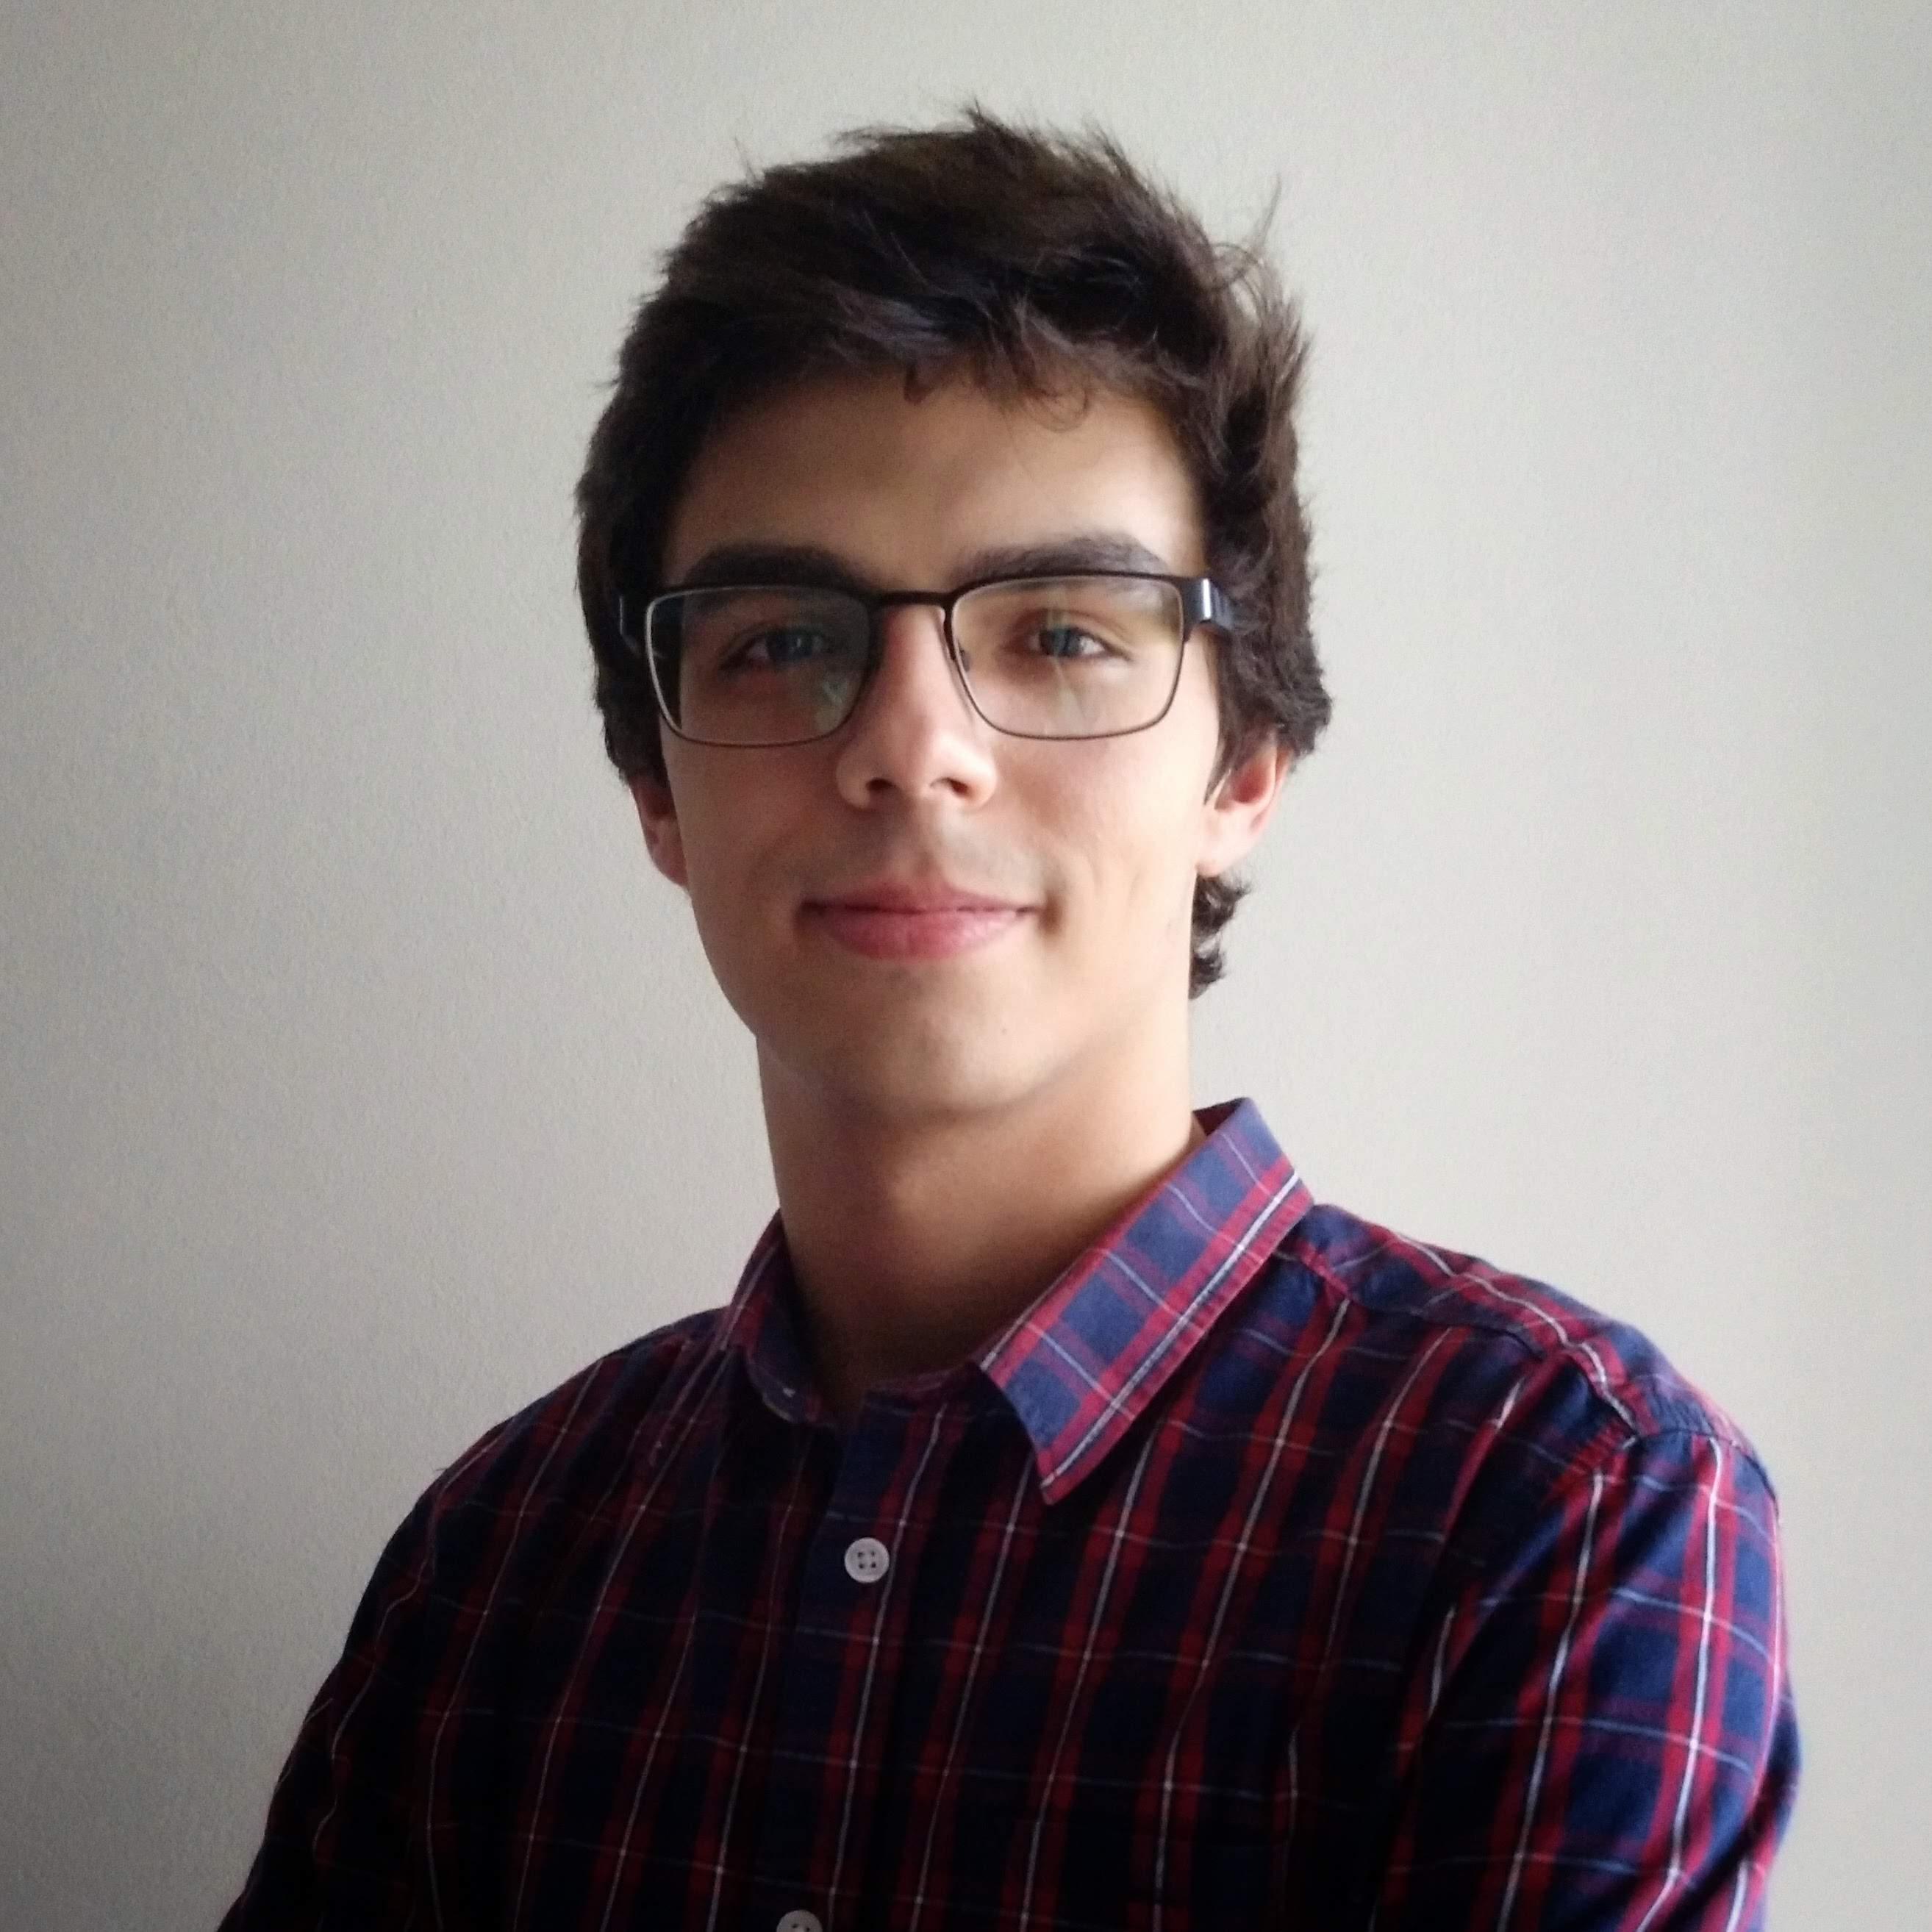
\includegraphics[width=1in,height=1.25in,clip,keepaspectratio]{me.jpeg}}]{Pedro Duarte}
I am currently pursuing my Master's Degree in Engineering studies at \ac{IST}, specializing in Intelligent Systems and Information Systems. My hobbies include photography and video-games. I strive to make this world a better place for everybody living in it and I am always ready to take on a challenge.
\end{IEEEbiography}

%%%%%%%%%%%%%%%%%%%%%%%%%%%%%%%%%%%%%%%%%%%%%%%%%%%%%%%%%%%%%%%%%%%%%%%%%%%%%%%%
%%%%%%%%%%%%%%%%%%%%%%%%%%%%%%%%%%%%%%%%%%%%%%%%%%%%%%%%%%%%%%%%%%%%%%%%%%%%%%%%
% *** DEFINITION OF ACRONYMS ***
	\acrodef{CPU}{Central Processing Unit}
	\acrodef{GUI}{Graphical User Interface}
	\acrodef{HTTP}{Hypertext Transfer Protocol}
	\acrodef{IST}{Instituto Superior Técnico}	
	\acrodef{LAN}{Local Area Network}
	\acrodef{PC}{Personal Computer}
	\acrodef{URL}{Uniform Resource Locator}
	\acrodef{VoD}{Video-on-demand}
	\acrodefplural{VoD}[VoDs]{Videos-on-demand}
	\acrodef{VoIP}{Voice over IP}
	\acrodef{WAN}{Wide Area Network}
	\acrodef{WLAN}{Wireless Local Area Network}
	\acrodef{WWAN}{Wireless Wide Area Network}
	\acrodef{WWW}{World Wide Web}
	
% that's all folks
\end{document}